\documentclass[17pt]{beamer} %Makes presentation
%\documentclass[handout]{beamer} %Makes Handouts
\usetheme{Singapore} %Gray with fade at top
\useoutertheme[subsection=false]{miniframes} %Supppress subsection in header
\useinnertheme{rectangles} %Itemize/Enumerate boxes
\usecolortheme{seagull} %Color theme
\usecolortheme{rose} %Inner color theme

\definecolor{light-gray}{gray}{0.75}
\definecolor{dark-gray}{gray}{0.55}
\setbeamercolor{item}{fg=light-gray}
\setbeamercolor{enumerate item}{fg=dark-gray}

\setbeamertemplate{navigation symbols}{}
%\setbeamertemplate{mini frames}[default]
%\setbeamercovered{dynamics}
\setbeamerfont*{title}{size=\Large,series=\bfseries}
\setbeamerfont{footnote}{size=\tiny}

%\setbeameroption{notes on second screen} %Dual-Screen Notes
%\setbeameroption{show only notes} %Notes Output

\setbeamertemplate{frametitle}{\vspace{.5em}\bfseries\insertframetitle}
\newcommand{\heading}[1]{\noindent \textbf{#1}\\ \vspace{1em}}

\usepackage{bbding,color,multirow,times,ccaption,tabularx,graphicx,verbatim,booktabs}
\usepackage{colortbl} %Table overlays
\usepackage[english]{babel}
%\usepackage[latin1]{inputenc}
%\usepackage[T1]{fontenc}
\usepackage{lmodern}

%\author[]{Thomas J. Leeper}
\institute[]{
  \inst{}%
  Department of Government\\London School of Economics and Political Science
}

\usepackage{tikz}
\usetikzlibrary{shapes,arrows}
\usetikzlibrary{decorations.pathreplacing}

\title{Getting to Regression: The Workhorse of Quantitative Political Analysis}


\date[]{}

\begin{document}

\frame{\titlepage}

\frame{\tableofcontents}

\section{Exam Preparation}
\frame{\tableofcontents[currentsection]}

\frame{
	
	\begin{center}
	\Large
	\textbf{What do you think will be on the exam?}
	\end{center}
	
}


\frame{}


\section{Correlation}
\frame{\tableofcontents[currentsection]}


\frame{
\frametitle{Correlation as Measure of Bivariate Relationship}

\begin{itemize}\itemsep1em
\item<1-> Covariance:\\
	$Cov(X,Y) = \sum_{i=1}^{n} \dfrac{(X_i - \bar{X})(Y_i - \bar{Y})}{n-1}$
\item<2-> Correlation:\\
	{\small 
	$Corr(X,Y) = r_{x,y} = \sum_{i=1}^{n} \dfrac{(X_i - \bar{X})(Y_i - \bar{Y})}{(n-1)s_x s_y}$
	
	where $s_x = \sqrt{\sum_{i=1}^{n}(x_i - \bar{x})^2}$
	}
\end{itemize}
}


\frame{

\frametitle{Correlation is linear!}

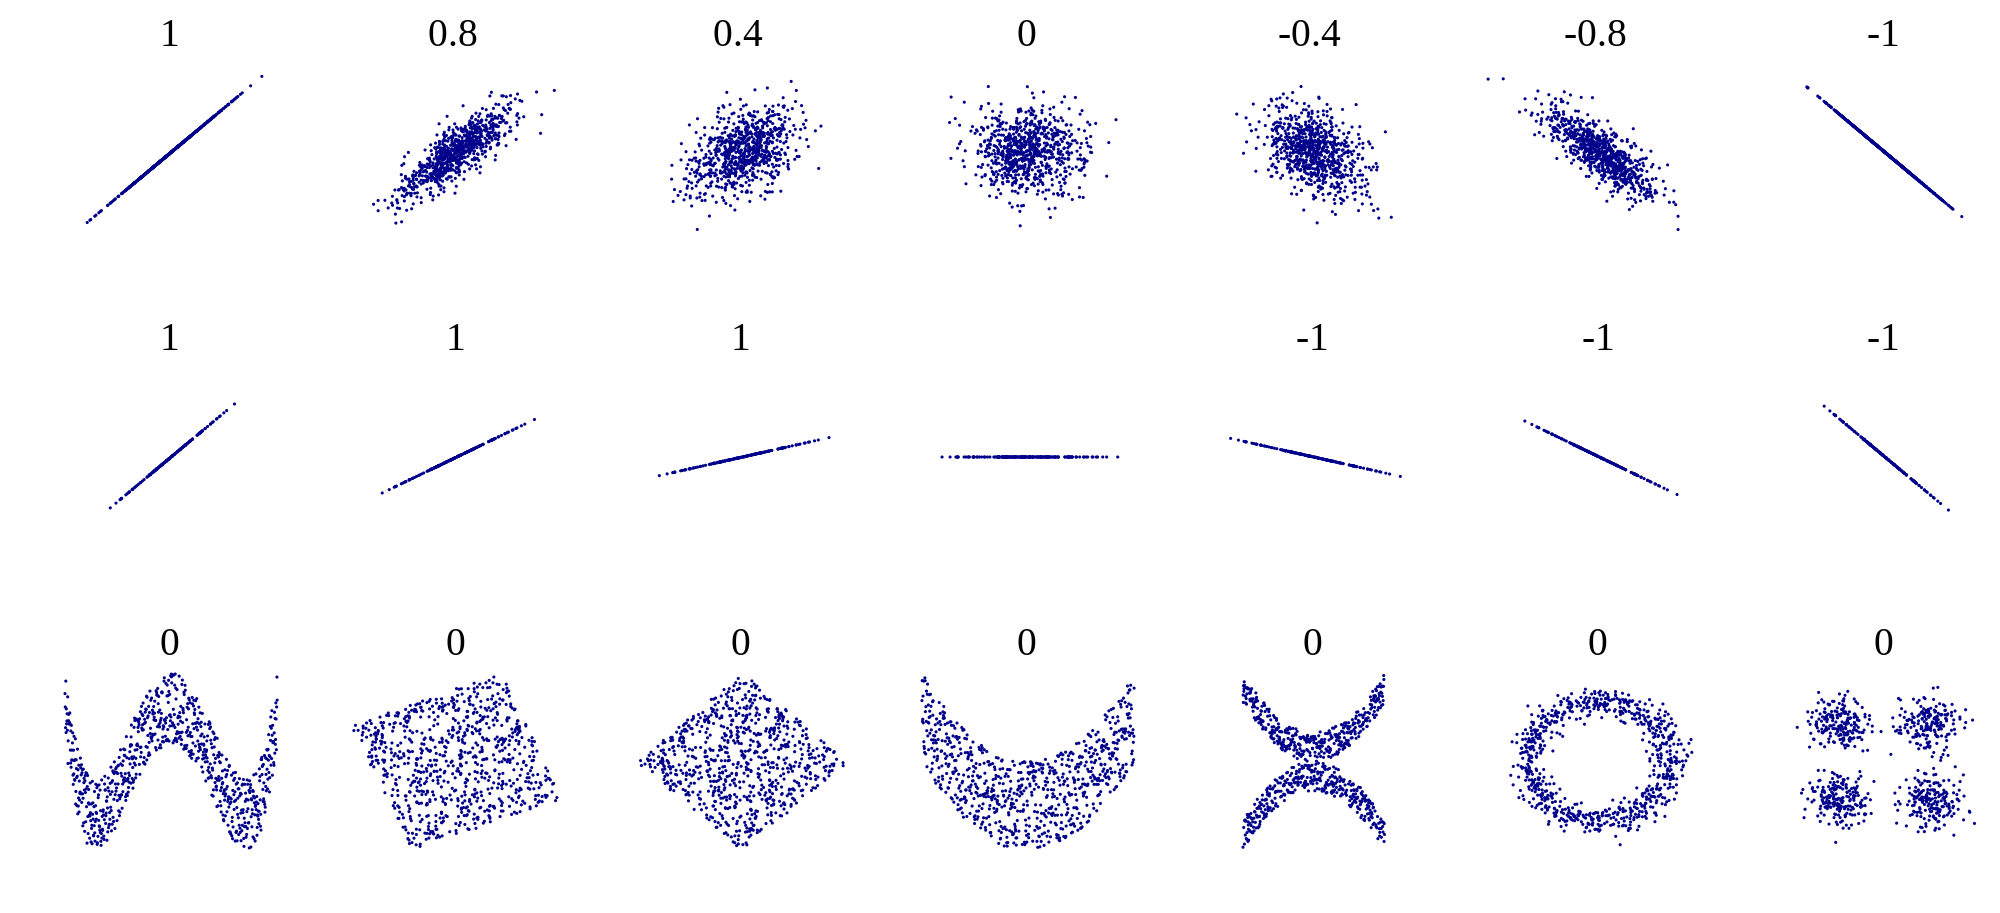
\includegraphics[width=\textwidth]{images/correlation}

\vspace{1em}
{\footnotesize Source: \href{https://commons.wikimedia.org/wiki/File:Correlation_examples2.svg}{Wikimedia}}
}

\frame{
	\frametitle{Guess the Correlation!}
	\begin{enumerate}\itemsep0.5em
	\item Go to: {\small \url{http://guessthecorrelation.com/}}
	\item Play a few rounds
	\end{enumerate}

}


\section{Regression}
\frame{\tableofcontents[currentsection]}

\frame{
	\frametitle{Regression}
	\begin{itemize}\itemsep1em
	\item Definition: a statistical method for measuring the relationships between one variable and many other variables
	\item<2-> Uses of Regression
		\begin{enumerate}\small
		\item Description
		\item Prediction
		\item Causal Inference
		\end{enumerate}
	\item<3-> \textit{Ordinary least squares} (OLS) regression
	\end{itemize}
}


\frame[label=ways]{
	\frametitle{Interpretations of OLS}
	\begin{enumerate}\itemsep1em
    	\item<2-> Line (or surface) of best fit
    	\item<2-> Ratio of $Cov(X,Y)$ and $Var(X)$
    	\item<2-> Minimizing residual sum of squares (SSR)
    	\item<3-> Estimating Unit-level Causal Effect
	\end{enumerate}
}


\frame{
	\frametitle{Bivariate Regression I}
	\begin{itemize}\itemsep1em
	\item $Y$ is continuous
	\item $X$ is a randomized treatment indicator/dummy $(0,1)$
	\item How do we know if the treatment $X$ had an effect on $Y$?
	\item<2-> Look at mean-difference: $E[Y_i|X_i=1] - E[Y_i|X_i=0]$
	\end{itemize}
}


\frame<1-2>[label=dummy]{
	\frametitle{Bivariate Regression I}
	\begin{itemize}\itemsep1em
    	\item Mean difference ($E[Y_i|X_i=1] - E[Y_i|X_i=0]$) is the regression line slope
    	\item Slope ($\beta$) defined as $\frac{\Delta Y}{\Delta X}$
    		\vspace{1em}
    		\begin{itemize}\itemsep1em
        		\item<2-> $\Delta Y = E[Y_i|X=1] - E[Y_i|X=0]$
        		\item<2-> $\Delta X = 1 - 0 = 1$
    		\end{itemize}
	\end{itemize}

}

\frame{
	\frametitle{Three Equations}
	\begin{enumerate}\itemsep1em
	\item Population:\\ $Y = \beta_0 + \beta_1 X \hspace{0.5em} (+ \epsilon)$
	\item<2-> Sample estimate:\\$\hat{y} = \hat{\beta}_0 + \hat{\beta}_1 x + e$
	\item<3-> Unit:
		\begin{align*}
		y_i & = \hat{\beta}_0 + \hat{\beta}_1 x_i + e_i\\
		    & = \bar{y}_{0i} + (y_{1i} - y_{0i}) x_i + (y_{0i} - \bar{y}_{0i})
		\end{align*}
	\end{enumerate}
}

\frame<1-6>[label=math]{
	\frametitle{Minimum Mathematical Requirements}
	\begin{enumerate}\itemsep1em
    	\item<1-> Do we need variation in $X$?
    		\begin{itemize}
        		\item<2-> Yes, otherwise dividing by zero
    		\end{itemize}
    	\item<3-> Do we need variation in $Y$?
    		\begin{itemize}
        		\item No, $\hat{\beta}_1$ can equal zero
    		\end{itemize}
    	\item<5-> How many observations do we need?
    		\begin{itemize}
    		\item<6-> $n \ge k$, where $k$ is number of parameters to be estimated
    		\end{itemize}
    	\item<7-> Can we have highly correlated regressors?
    		\begin{itemize}
    		\item<8-> Generally no (due to multicollinearity)
    		\end{itemize}
	\end{enumerate}
}


\frame[label=bivariate1]{
	\begin{center}
	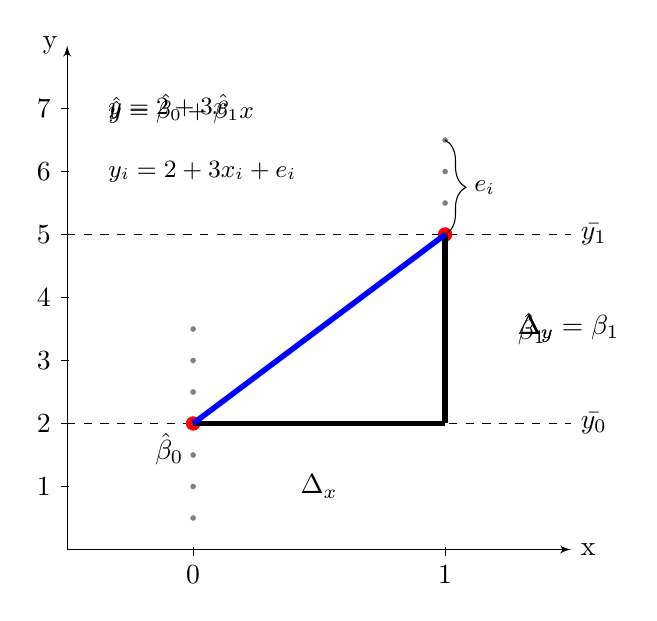
\begin{tikzpicture}[>=latex', scale=0.8]
        \draw[->] (0,0) node[below] (origin) {}  -- (8,0) node[right] (xaxis) {x};
        \draw[->] (origin) -- (0,8) node[left] (yaxis) {y};
        % x ticks
        \draw (2,1pt) -- (2,-3pt) node[anchor=north] {0};
        \draw (6,1pt) -- (6,-3pt) node[anchor=north] {1};
        % y ticks
        \foreach \y in {1,...,7}
             \draw (1pt,\y) -- (-3pt,\y) node[anchor=east] {$\y$};
        
        % points
        \foreach \y in {0.5,1.0,...,3.5} {
        	\draw[gray,fill] (2,\y) circle [radius=1pt];
        	\draw[gray,fill] (6,3+\y) circle [radius=1pt];
        }
        % y_0-bar
        \draw<2-4>[dashed] (0,2) -- (8,2) node[right] {$\bar{y_0}$};
        % y_1-bar
        \draw<2-4>[dashed] (0,5) -- (8,5) node[right] {$\bar{y_1}$};
        % mean points
        \draw<2->[red,fill] (2,2) circle [radius=3pt];
        \draw<2->[red,fill] (6,5) circle [radius=3pt];
        
        % slope
        \draw<3-4>[solid, line width=2pt] (2,2) -- (6,2);
        \draw<3-5>[solid, line width=2pt] (6,2) -- (6,5);
        \node<3-4>(deltax) at (4,1) {$\Delta_x$};
        \node<3>[right](deltay) at (7,3.5) {$\Delta_y$};
        \node<4>[right](deltay) at (7,3.5) {$\Delta_y = \beta_1$};
        \node<5>[right](deltay) at (7,3.5) {$\hat{\beta}_1$};
        
        \draw<4->[blue, solid, line width=2pt] (2,2) -- (6,5);
        \node<4-5>[below left](b0) at (2,2) {$\hat{\beta}_0$};
        
        \node<5>[right](eq) at (0.5,7) {\small $\hat{y} = \hat{\beta}_0 + \hat{\beta}_1 x$};
        \node<6->[right](eq) at (0.5,7) {\small $\hat{y} = 2 + 3 x$};
        \node<7->[right](eq) at (0.5,6) {\small $y_i = 2 + 3 x_i + e_i$};
        \draw<7->[right,decorate,decoration={brace,mirror,amplitude=7.5pt}] (6,5)  -- (6,6.5)
        	node [right, pos=0.5, xshift=7] {\small $e_i$};
    \end{tikzpicture}
    \end{center}
}


\frame[label=calculations]{
	\frametitle{Calculations}
	
	\small
	If $x$ is continuous, calculation is more complicated:\\
	$\widehat{\beta_1} = Cov(x,y) / Var(x)$
	
	\vspace{1em}
	\begin{tabular}{rrrrrr} \hline
	$x_i$ & $y_i$ & $x_i - \bar{x}$ & $y_i - \bar{y}$ & $(x_i - \bar{x})(y_i - \bar{y})$ & $(x_i - \bar{x})^2$\\ \hline
	1 & 1 & ? & ? & ? & ? \\
	2 & 5 & ? & ? & ? & ? \\
	3 & 3 & ? & ? & ? & ? \\
	4 & 6 & ? & ? & ? & ? \\
	5 & 2 & ? & ? & ? & ? \\
	6 & 7 & ? & ? & ? & ? \\ \hline
	$\bar{x}$ & $\bar{y}$ & & & $Cov(x,y)$ & $Var(x)$ \\ \hline
	\end{tabular}
}

\frame<1-5>[label=scatter]{
	\begin{center}
	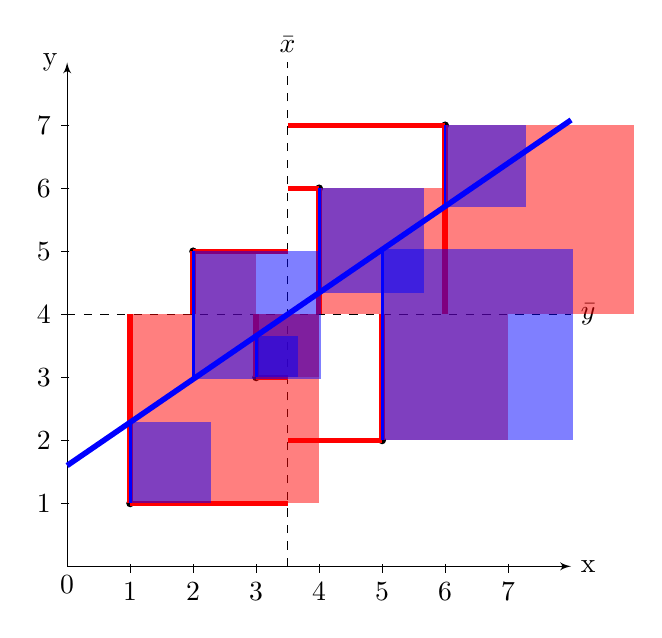
\begin{tikzpicture}[>=latex', scale=0.8]
        \draw[->] (0,0) node[below] (origin) {0}  -- (8,0) node[right] (xaxis) {x};
        \draw[->] (origin) -- (0,8) node[left] (yaxis) {y};
        % x ticks
        \foreach \x in {1,...,7}
        	\draw (\x,1pt) -- (\x,-3pt) node[anchor=north] {$\x$};
        % y ticks
        \foreach \y in {1,...,7}
             \draw (1pt,\y) -- (-3pt,\y) node[anchor=east] {$\y$};
        % points
        \draw[fill] (1,1) circle [radius=1.5pt];
        \draw[fill] (2,5) circle [radius=1.5pt];
        \draw[fill] (3,3) circle [radius=1.5pt];
        \draw[fill] (4,6) circle [radius=1.5pt];
        \draw[fill] (5,2) circle [radius=1.5pt];
        \draw[fill] (6,7) circle [radius=1.5pt];
        % x-bar
        \draw<2->[dashed] (3.5, 0) -- (3.5,8) node[above] {$\bar{x}$};
        % y-bar
        \draw<2->[dashed] (0,4) -- (8,4) node[right] {$\bar{y}$};
        
        % x-deviations
        \draw<3>[red, line width=2pt] (1,1) -- (3.5,1);
        \draw<3>[red, line width=2pt] (2,5) -- (3.5,5);
        \draw<3>[red, line width=2pt] (3,3) -- (3.5,3);
        \draw<3>[red, line width=2pt] (4,6) -- (3.5,6);
        \draw<3>[red, line width=2pt] (5,2) -- (3.5,2);
        \draw<3>[red, line width=2pt] (6,7) -- (3.5,7);
        % y-deviations
        \draw<4,6-7,10-11>[red, line width=2pt] (1,1) -- (1,4);
        \draw<4,6-7,10-11>[red, line width=2pt] (2,5) -- (2,4);
        \draw<4,6-7,10-11>[red, line width=2pt] (3,3) -- (3,4);
        \draw<4,6-7,10-11>[red, line width=2pt] (4,6) -- (4,4);
        \draw<4,6-7,10-11>[red, line width=2pt] (5,2) -- (5,4);
        \draw<4,6-7,10-11>[red, line width=2pt] (6,7) -- (6,4);
        
		\fill<7,11>[red, opacity=0.5] (1,1) rectangle (4,4);
		\fill<7,11>[red, opacity=0.5] (2,5) rectangle (3,4);
		\fill<7,11>[red, opacity=0.5] (3,3) rectangle (4,4);
		\fill<7,11>[red, opacity=0.5] (4,6) rectangle (6,4);
		\fill<7,11>[red, opacity=0.5] (5,2) rectangle (7,4);
		\fill<7,11>[red, opacity=0.5] (6,7) rectangle (9,4);

        % line
        \draw<5->[blue, line width=2pt] (0,1.6) -- (8,7.0856);
        
        % residuals
        \draw<8->[blue, line width=1pt] (1,1) -- (1,2.29);
        \draw<8->[blue, line width=1pt] (2,5) -- (2,2.97);
        \draw<8->[blue, line width=1pt] (3,3) -- (3,3.66);
        \draw<8->[blue, line width=1pt] (4,6) -- (4,4.34);
        \draw<8->[blue, line width=1pt] (5,2) -- (5,5.03);
        \draw<8->[blue, line width=1pt] (6,7) -- (6,5.71);
		
		\fill<9-11>[blue, opacity=0.5] (1,1) rectangle (2.29,2.29);
		\fill<9-11>[blue, opacity=0.5] (2,5) rectangle (4.03,2.97);
		\fill<9-11>[blue, opacity=0.5] (3,3) rectangle (3.66,3.66);
		\fill<9-11>[blue, opacity=0.5] (4,6) rectangle (5.66,4.34);
		\fill<9-11>[blue, opacity=0.5] (5,2) rectangle (8.03,5.03);
		\fill<9-11>[blue, opacity=0.5] (6,7) rectangle (7.29,5.71);

		
    \end{tikzpicture}
    \end{center}
}


\againframe{calculations}

% mean(x) = 3.5
% mean(y) = 4
% cov(x,y) = 11
% var(x) = 17.5
% slope = 0.627

\frame[label=calculations2]{
	\frametitle{Calculations}
	
	\small
	If $x$ is continuous, calculation is more complicated:\\
	\only<1>{$\widehat{\beta_1} = Cov(x,y) / Var(x)$}\only<2>{$\widehat{\beta_1} = Cov(x,y) / Var(x) = 11/17.5 = \mathbf{0.627}$}
	
	\vspace{1em}
	\begin{tabular}{rrrrrr} \hline
	$x_i$ & $y_i$ & $x_i - \bar{x}$ & $y_i - \bar{y}$ & $(x_i - \bar{x})(y_i - \bar{y})$ & $(x_i - \bar{x})^2$\\ \hline
	1 & 1 & $-2.\bar{6}$ & -3 & $-6.6\bar{6}$ & 6.25 \\
	2 & 5 & $-1.\bar{3}$ & +1 & $-2.00$ & 2.25 \\
	3 & 3 & $-0.\bar{6}$ & -1 & $-0.3\bar{3}$ & 0.25 \\
	4 & 6 & $+0.\bar{3}$ & +2 & $-0.1\bar{6}$ & 0.25 \\
	5 & 2 & $+1.\bar{6}$ & -2 & $-2.50$ & 2.25 \\
	6 & 7 & $+2.\bar{3}$ & +3 & $-8.3\bar{3}$ & 6.25 \\ \hline
	3.5 & $3.\bar{6}$ & & & 11 & 17.5 \\ \hline
	\end{tabular}
}


\frame{
	\frametitle{Intercept $\hat{\beta}_0$}
	\begin{itemize}\itemsep1em
	\item Simple formula: $\hat{\beta}_0 = \bar{y} - \hat{\beta}_1 \bar{x}$
	\item<2-> Intuition: OLS fit always runs through point $(\bar{x}, \bar{y})$
	\item<3-> Ex.: $\hat{\beta}_0 = 3.\bar{6} - 0.627 * 3.5 = 1.4\bar{6}$
	\item<4-> $\hat{y} = 1.4\bar{6} + 0.6857 \hat{x}$
	\end{itemize}
}

\againframe<5>{scatter}

\frame{
	\frametitle{Systematic versus unsystematic components}
	\begin{itemize}\itemsep1em
    	\item<2-> Systematic: Regression line (slope)
    		\begin{itemize}
    		\item Linear regression estimates the conditional means of the population data (i.e., $E[Y|X]$)
    		\end{itemize}
    	\item<3-> Unsystematic: Error term is the deviation of observations from the line
    		\begin{itemize}
        		\item The difference between each value $y_i$ and $\hat{y}_i$ is the \textit{residual}: $e_i$
        		\item OLS produces an estimate of $\beta$ that minimizes the \textit{residual sum of squares}
    		\end{itemize}
	\end{itemize}
}

\frame{
	\frametitle{Why are there residuals?}
	\begin{itemize}\itemsep1em
		\item<2-> Fundamental randomness
		\item<3-> Measurement error
		\item<4-> Omitted variables
	\end{itemize}
}

\frame{
	\frametitle{OLS Minimizes SSR}
	\begin{itemize}\itemsep1em
    	\item Total Sum of Squares (SST): $\sum_{i=1}^{n}(y_i - \bar{y})^2$
    	\item We can partition SST into two parts (ANOVA):
    		\begin{itemize}
    		\item Explained Sum of Squares (SSE)
    		\item Residual Sum of Squares (SSR)
    		\end{itemize}
    	\item $SST = SSE + SSR$
    	\item OLS is the line with the lowest SSR
	\end{itemize}
}

\againframe<5-11>{scatter}

\frame{
	\frametitle{RMSE ($\sigma$)}
	\begin{itemize}
	\item Definition: $\hat{\sigma} = \sqrt{\frac{SSR}{n-p}}$, where $p$ is number of parameters estimated
	\item Interpretation:
		\begin{itemize}
		\item How far, on average, are the observed $y$ values from their corresponding fitted values $\hat{y}$
		\item $sd(y)$ is how far, on average, a given $y_i$ is from $\bar{y}$
		\item $\sigma$ is how far, on average, a given $y_i$ is from $\hat{y}_i$
		\end{itemize}
	\item Units: same as $y$ (range 0 to $sd(y)$)
	\end{itemize}
}


\frame{
	\frametitle{Correlation/Regression Equivalence}
	\begin{itemize}\itemsep1em
	\item Definition: $Corr(x,y) = \hat{r}_{x,y} = \frac{Cov(x,y)}{(n-1) s_x s_y}$
	\item Slope $\hat{\beta}_1$ and correlation $\hat{r}_{x,y}$ are simply different scalings of $Cov(x,y)$
	\vspace{1em}
	\item<2-> $R^2 = \hat{r}_{x,y}^2 = \frac{SSE}{SST} = 1 - \frac{SSR}{SST}$
	\end{itemize}
}


\frame{\frametitle{Questions about OLS calculations?}}


\frame[label=anygood]{
	\frametitle{Are Our Estimates Any Good?}
	\begin{enumerate}\itemsep1em
   		\item<2-> Works mathematically
   		\item<2-> Linear relationship between $X$ and $Y$
   		\item<2-> $X$ is measured without error
   		\item<2-> No missing data (or MCAR)
   		\item<2-> No confounding (next week)
	\end{enumerate}
}


\frame{
	\frametitle{Linear Relationship}
	\begin{itemize}\itemsep1em
    	\item If linear, no problems
    	\item If non-linear, we need to transform
    		\begin{itemize}
        		\item Power terms (e.g., $x^2$, $x^3$)
        		\item log (e.g., $log(x)$)
        		\item Other transformations
        		\item If categorical: convert to set of indicators
        		\item Multivariate interactions (next week)
    		\end{itemize}
	\end{itemize}
}

\frame{
	\frametitle{Coefficient Interpretation Activity}
	\begin{itemize}\itemsep1em
	\item Four types of variables:
		\begin{enumerate}
		\item Indicator (0,1)
		\item Categorical
		\item Ordinal
		\item Interval
		\end{enumerate}
	\item How do we interpret a coefficient on each of these types of variables?
	\end{itemize}
}


\frame{\large Questions?}


\frame{}


\end{document}
